% =============================================================================
% CAPÍTULO 3 --- COMPONENTE 1: BANCO DE DADOS INTEGRADO E PIPELINE DE GERAÇÃO
% Versão revisada segundo o guideline editorial da tese BioRemPP
% =============================================================================

\chapter{Componente 1: banco de dados integrado e pipeline de geração}
\label{cap:comp1}

% -----------------------------------------------------------------------------
\section{Motivação e escopo do componente}
\label{sec:c1-motivacao}
% -----------------------------------------------------------------------------

O banco integrado fornece a base de dados usada pelos demais componentes do ecossistema \biorempp{}. As fontes consideradas neste trabalho organizam dimensões distintas da evidência relevante para a biorremediação. O \gls{kegg} descreve relações entre compostos, grupos de ortologia KEGG, enzimas e reações; o \gls{hadeg} reúne anotações especializadas em degradação aeróbica de hidrocarbonetos; o \gls{toxcsm} fornece predições toxicológicas indexadas por composto; e as fontes institucionais identificam substâncias submetidas a processos de priorização, regulamentação ou classificação. Como essas fontes usam diferentes unidades de observação e sistemas de identificação, nenhuma delas, isoladamente, reúne o conjunto de evidências associado a um composto prioritário.

O \biorempp{} organiza essas informações por meio de uma estrutura centrada no composto (\textit{compound-centric}). O universo inicial da integração corresponde aos compostos presentes em sete fontes institucionais Esse recorte restringe a integração às substâncias contempladas por fontes de priorização, regulamentação ou classificação, em vez de incorporar todos os compostos disponíveis nas bases funcionais e toxicológicas. Cada composto permanece associado a uma ou mais referências institucionais, permitindo distinguir a evidência biológica da origem institucional de sua priorização ou classificação.

A tabela central, o pipeline de geração e as camadas de validação constituem o mesmo componente científico. Cada versão do banco é produzida a partir dos arquivos curados de entrada, do snapshot versionado das relações recuperadas do KEGG, do esquema público de dados e dos relatórios de validação. Em conjunto, esses artefatos registram o processo de produção do banco, permitem rastrear as transformações intermediárias e tornam explícitas as diferenças entre versões.

% -----------------------------------------------------------------------------
\section{Fontes de dados e proveniência}
\label{sec:c1-fontes}
% -----------------------------------------------------------------------------

A construção do componente envolve três níveis de proveniência e integração. O primeiro delimita o universo de compostos prioritários a partir de fontes institucionais. O segundo reúne as entradas curadas e as relações recuperadas programaticamente para produzir a tabela central BioRemPP. O terceiro corresponde aos conjuntos funcionais e toxicológicos ligados à tabela central pelos identificadores \gls{ko} e \gls{cpd}. Essa separação distingue as fontes usadas na construção do banco dos conjuntos de dados produzidos ou integrados pelo próprio ecossistema.

\subsection{Universo regulatório de compostos prioritários}

O universo inicial foi definido por sete fontes institucionais de priorização, regulamentação ou classificação de substâncias. A \gls{iarc} foi representada por três categorias de carcinogenicidade, resultando em nove valores controlados no campo \texttt{referenceAG} (Tabela~\ref{tab:c1-regulatory-sources}). Cada ocorrência de um composto em uma dessas fontes foi preservada como associação independente. Assim, uma mesma substância pode permanecer vinculada a mais de uma referência institucional.

A curadoria da identidade química considerou nomes, números \gls{cas} e sinônimos empregados nas listas de origem. Os registros foram incorporados quando a identidade química pôde ser associada de forma inequívoca a um identificador KEGG Compound. Na versão 1.1.0, a proveniência institucional é representada principalmente pelos pares \texttt{cpd}--\texttt{referenceAG} presentes no conjunto curado de compostos regulados.

\begin{table}[htbp]
\centering
\caption{Fontes institucionais usadas para definir o universo de compostos prioritários do \biorempp{}. Os nove códigos de \texttt{referenceAG} correspondem a sete fontes, com a IARC representada por três categorias de carcinogenicidade.}
\label{tab:c1-regulatory-sources}
\footnotesize
\begin{tabularx}{\textwidth}{@{}lXlX@{}}
\toprule
\textbf{Código} & \textbf{Fonte institucional} & \textbf{Escopo} & \textbf{Função no recorte} \\
\midrule
ATSDR
& Agency for Toxic Substances and Disease Registry
& EUA
& Inclui substâncias associadas a riscos para a saúde pública e a locais contaminados. \\

EPA
& U.S. Environmental Protection Agency
& EUA
& Inclui contaminantes contemplados por programas e referências ambientais dos Estados Unidos. \\

CONAMA
& Conselho Nacional do Meio Ambiente
& Brasil
& Inclui contaminantes contemplados por normas ambientais brasileiras. \\

WFD
& Water Framework Directive
& União Europeia
& Inclui substâncias prioritárias relacionadas à qualidade das águas. \\

EPC
& Environmental Priority Chemicals
& Europa
& Inclui substâncias priorizadas em avaliações ambientais europeias. \\

PSL
& Priority Substances List, sob a CEPA
& Canadá
& Inclui substâncias submetidas à priorização no contexto canadense. \\

IARC1
& IARC Group 1, Carcinogenic to humans
& Internacional
& Identifica compostos classificados como carcinogênicos para humanos. \\

IARC2A
& IARC Group 2A, Probably carcinogenic to humans
& Internacional
& Identifica compostos classificados como provavelmente carcinogênicos para humanos. \\

IARC2B
& IARC Group 2B, Possibly carcinogenic to humans
& Internacional
& Identifica compostos classificados como possivelmente carcinogênicos para humanos. \\
\bottomrule
\end{tabularx}
\end{table}

O recorte institucional funciona como critério de inclusão para as evidências funcionais e toxicológicas. Em vez de reunir todos os compostos disponíveis nas fontes consultadas, o banco concentra-se em substâncias cuja relevância ambiental ou sanitária foi formalmente registrada. As sobreposições entre listas e categorias são preservadas, permitindo identificar compostos priorizados por mais de uma instituição ou jurisdição.

\subsection{Entradas locais do pipeline}

O pipeline usa seis arquivos locais, cujas funções estão resumidas na Tabela~\ref{tab:c1-local-inputs}. Os nomes correspondem aos arquivos exigidos pelo contrato de entrada versionado da versão 1.1.0.

\begin{table}[htbp]
\centering
\caption{Arquivos locais usados na geração do banco BioRemPP v1.1.0.}
\label{tab:c1-local-inputs}
\small
\begin{tabularx}{\textwidth}{@{}lX@{}}
\toprule
\textbf{Arquivo} & \textbf{Função no pipeline} \\
\midrule
\texttt{kegglistcompounds.xlsx}
& Integra o conjunto local de compostos exigido pelo contrato de entrada. Os valores públicos de \texttt{compoundname} são atualizados a partir da lista recuperada do KEGG. \\

\texttt{curated\_regulated\_compounds.xlsx}
& Armazena as associações normalizadas entre \texttt{cpd} e \texttt{referenceAG} que delimitam o universo institucional principal. \\

\texttt{curated\_programatic\_missing\_compounds.xlsx}
& Acrescenta associações curadas entre \texttt{cpd} e \texttt{ko} que não foram recuperadas integralmente pelas relações programáticas. A referência institucional é incorporada por correspondência com o universo regulatório. \\

\texttt{curated\_compound\_classes.xlsx}
& Associa os compostos ao vocabulário controlado do campo \texttt{compoundclass}. \\

\texttt{kegglistko.txt}
& Fornece as informações usadas no preenchimento dos campos \texttt{genesymbol} e \texttt{genename}. \\

\texttt{curated\_enzyem\_names\_extracted.txt}
& Fornece os termos curados usados na atribuição dos descritores do campo \texttt{enzyme\_activity}. \\
\bottomrule
\end{tabularx}
\end{table}

Antes das transformações, o pipeline verifica a presença e a estrutura mínima desses arquivos. O conteúdo validado é reunido em uma representação intermediária que preserva separadamente os compostos regulados, as associações curadas entre composto e KO, as classes químicas, as informações dos KOs e o vocabulário de descritores enzimáticos. Essa etapa estabelece a fronteira entre os dados locais curados e as relações recuperadas do KEGG.

\subsection{Aquisição programática e proveniência do KEGG}

As relações funcionais são recuperadas por consultas ao KEGG REST API. As operações usadas pelo pipeline podem ser agrupadas em três funções: obtenção das relações entre compostos, KOs, números EC e reações; recuperação dos nomes de compostos e das descrições de reações; e registro da versão do KEGG consultada (Tabela~\ref{tab:c1-kegg-endpoints}).

\begin{table}[htbp]
\centering
\caption{Grupos de consultas ao KEGG REST usados na geração da tabela central BioRemPP v1.1.0.}
\label{tab:c1-kegg-endpoints}
\small
\begin{tabularx}{\textwidth}{@{}lX@{}}
\toprule
\textbf{Grupo de consultas} & \textbf{Informação recuperada} \\
\midrule
Relações funcionais
& Associações KO--EC, KO--reação, composto--EC, composto--reação e EC--reação. \\

Descrições e nomenclatura
& Identificadores, nomes de compostos e descrições textuais das reações KEGG. \\

Metadados de proveniência
& Versão da base KEGG e data associada à consulta executada. \\
\bottomrule
\end{tabularx}
\end{table}

As respostas foram normalizadas antes da integração. Os prefixos próprios do KEGG foram removidos, e os identificadores de compostos, KOs e reações foram verificados segundo seus padrões formais de Regex.

As consultas foram executadas com política configurável de repetição e tratamento de falhas transitórias. Respostas não recuperáveis interromperam a etapa de aquisição, evitando a produção do banco a partir de relações incompletas sem registro explícito. As relações normalizadas foram preservadas como estado intermediário para uso nas etapas posteriores de integração e validação.

A versão 1.1.0 foi construída a partir do KEGG Release 118.0+, consultado em 18 de maio de 2026. A versão da fonte, a data da consulta e sua origem foram registradas nos metadados da execução. Os endpoints individuais, os parâmetros de aquisição, os formatos dos artefatos intermediários e os procedimentos de reconstrução estão descritos na documentação oficial dos repositórios da organização BioRemPP, disponível em \url{https://github.com/BioRemPP}.

\subsection{Conjuntos de dados integrados ao ecossistema}

A camada de dados do ecossistema reúne a tabela central BioRemPP e três conjuntos complementares: HADEG, o subconjunto KEGG Xenobiotics Metabolism and Degradation e ToxCSM (Tabela~\ref{tab:c1-fontes}). Esses conjuntos permanecem estruturalmente separados e são relacionados por identificadores compartilhados. As fontes de evidência funcional são organizadas por \gls{ko}, enquanto as predições toxicológicas são indexadas por \gls{cpd}.

\begin{table}[htbp]
\centering
\caption{Conjuntos de dados disponíveis na camada integrada do \biorempp{} v1.1.0 e identificadores usados para estabelecer as relações entre eles.}
\label{tab:c1-fontes}
\small
\begin{tabular}{@{}lrrl@{}}
\toprule
\textbf{Conjunto de dados} & \textbf{Linhas} & \textbf{Colunas} & \textbf{Identificador de ligação} \\
\midrule
Tabela central BioRemPP & 123.543 & 11 & \gls{ko}, \gls{cpd} \\
HADEG                   &     867 &  4 & \gls{ko} \\
KEGG Degradation        &     855 &  3 & \gls{ko} \\
ToxCSM                  &     370 & 66 & \gls{cpd} \\
\bottomrule
\end{tabular}
\end{table}

A tabela central representa associações entre compostos prioritários, grupos de ortologia KEGG e referências institucionais. Cada linha contém uma combinação de \texttt{cpd}, \texttt{ko} e \texttt{referenceAG}, acrescida da classe e do nome do composto, das informações gênicas e do descritor de atividade enzimática. Quando sustentadas pelas relações recuperadas do KEGG, as colunas \texttt{ec}, \texttt{reaction} e \texttt{reaction\_description} registram a transformação enzimática associada. A ausência dessas relações é representada por \texttt{NA}, preservando a diferença entre uma associação parcialmente resolvida e uma relação funcional completa.

O \textbf{HADEG}~\citep{rojas2023hadeg} acrescenta anotações especializadas em degradação aeróbica de hidrocarbonetos, plásticos e produção de biosurfactantes. O conjunto contém 323 símbolos gênicos únicos, 337 \glspl{ko} e 71 vias metabólicas, distribuídas entre alcanos, aromáticos, alcenos, cicloalcanos, BTEX, Polímeros plásticos e classes de Biosurfactantes. A relação com a tabela central é estabelecida pelo identificador \gls{ko}.

O \textbf{subconjunto KEGG Xenobiotics Metabolism and Degradation}~\citep{kanehisa2022kegg} reúne 517 \glspl{ko} associados a 20 vias selecionadas do metabolismo de xenobióticos. Entre elas estão as vias relacionadas à degradação de naftaleno, benzoato, aminobenzoato, cloroalcanos, atrazina, bisfenol e hidrocarbonetos aromáticos policíclicos. Esse conjunto também é relacionado à tabela central por \gls{ko}.

O \textbf{ToxCSM}~\citep{desa2022toxCSM} fornece predições \gls{qsar} para 370 dos 384 compostos presentes no banco, correspondendo a 96,4\% de cobertura. Cada composto possui 31 endpoints, representados por uma categoria de risco (\textit{Safety}, \textit{Moderate Risk} ou \textit{High Risk}) e por um escore contínuo entre 0 e 1. Os endpoints abrangem toxicidade ambiental, genotoxicidade, toxicidade em órgãos, interação com receptores nucleares e ativação de respostas ao estresse.

A categoria ambiental reúne seis endpoints relacionados a aves, crustáceos, peixes, polinizadores, protozoários e biodegradação predita. A categoria de genotoxicidade compreende mutagenicidade no teste de Ames, carcinogenicidade e formação de micronúcleos. O grupo de toxicidade em órgãos contém oito endpoints, incluindo hepatotoxicidade, cardiotoxicidade mediada por hERG e efeitos oculares e dérmicos. Outros nove endpoints avaliam ligação ou modulação de receptores nucleares, incluindo AhR, AR, AR-LBD, ER, ER-LBD, aromatase, GR, PPAR-$\gamma$ e TR. Os cinco endpoints restantes representam ativação das vias ARE, ATAD5, HSE, MMP e p53.


% -----------------------------------------------------------------------------
\section{Modelo de organização relacional baseado em KO e CPD}
\label{sec:c1-dualaxis}
% -----------------------------------------------------------------------------

A organização dos conjuntos integrados é baseada em duas entidades de referência: grupos de ortologia KEGG, representados pelos identificadores \gls{ko}, e compostos químicos, representados pelos identificadores \gls{cpd} (Figura~\ref{fig:c1-dualaxis}). Essas entidades preservam as unidades de observação adotadas pelas fontes originais e permitem relacionar evidências funcionais e toxicológicas.

A entidade funcional, representada por \gls{ko}, relaciona a tabela central ao HADEG e ao subconjunto KEGG Degradation. Essa organização reúne as associações composto--KO do banco, as vias descritas pelo HADEG e os grupos de ortologia presentes nas vias selecionadas do metabolismo de xenobióticos.

A entidade química, representada por \gls{cpd}, relaciona a tabela central ao ToxCSM. Essa ligação preserva a indexação das predições toxicológicas por composto e permite consultar os endpoints associados a uma substância sem alterar a organização funcional baseada em KO.

\begin{figure}[htbp]
\centering
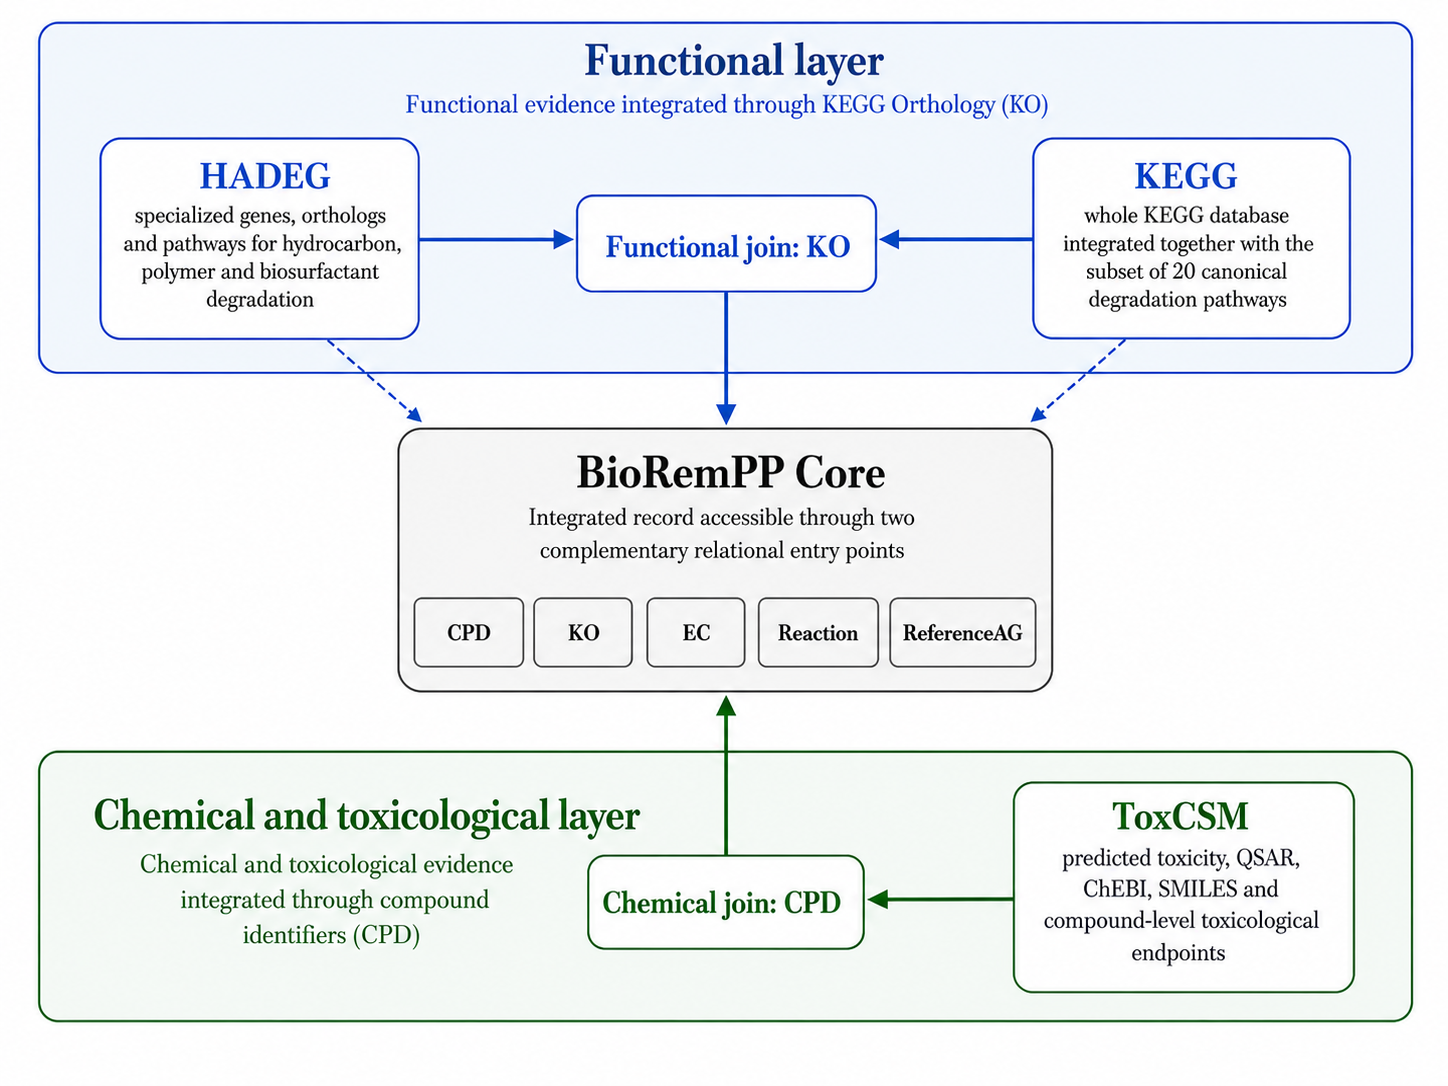
\includegraphics[width=\textwidth]{figures/chapter_03/fig_03_01_dual_axis.png}
\caption{Modelo de organização relacional do banco \biorempp{} baseado nas entidades KO e CPD. Os identificadores \gls{ko} relacionam as evidências funcionais, enquanto os identificadores \gls{cpd} relacionam as informações químicas e toxicológicas.}
\label{fig:c1-dualaxis}
\end{figure}

A manutenção das duas entidades decorre da estrutura das fontes integradas. A evidência funcional é organizada por grupos de ortologia KEGG, números EC e reações, enquanto as predições toxicológicas são indexadas por estrutura molecular. A conversão de todas as evidências para uma única chave exigiria relações que não estão disponíveis para todos os registros e poderia eliminar informações preservadas pelas fontes originais.

KO e CPD constituem, portanto, pontos de entrada complementares para consulta. O primeiro permite recuperar evidências relacionadas a funções gênicas e transformações enzimáticas. O segundo permite recuperar informações associadas ao composto, incluindo sua proveniência institucional e suas predições toxicológicas. Essa organização não pressupõe correspondência unívoca entre grupo de ortologia e composto.

\subsection{Estados de suporte relacional}

A construção da tabela central parte do universo de chaves
\texttt{cpd}--\texttt{ko}--\texttt{referenceAG}. Essas chaves são obtidas de
três origens: relações composto--EC--KO, relações composto--reação--KO e
associações composto--KO acrescentadas por curadoria. Cada chave é expandida
de acordo com as relações disponíveis no snapshot versionado do KEGG usado
na execução.

As chaves são classificadas em seis estados de suporte relacional, definidos
pela completude e pela origem das relações recuperadas
(Tabela~\ref{tab:c1-support-stages}). Os três primeiros estados resultam em
registros com número EC e reação preenchidos, embora usem caminhos distintos
de confirmação. Os dois estados seguintes preservam associações sustentadas
apenas por número EC ou por reação. O último mantém a associação curada entre
composto e KO quando as relações consultadas não permitem resolver nenhum
desses campos.

\begin{table}[htbp]
\centering
\caption{Estados de suporte usados na expansão das chaves
\texttt{cpd}--\texttt{ko}--\texttt{referenceAG}. Os identificadores internos
permitem relacionar as categorias descritas aos registros produzidos
pelo pipeline.}
\label{tab:c1-support-stages}
\small
\begin{tabularx}{\textwidth}{@{}p{3.2cm}p{2.8cm}Xll@{}}
\toprule
\textbf{Estado de suporte}
& \textbf{Identificador}
& \textbf{Critério de construção}
& \textbf{EC}
& \textbf{Reação} \\
\midrule

Mapeamento denso
& \texttt{dense}
& O KO possui número EC e reação, e a relação entre ambos é sustentada pelos
links EC--reação consultados.
& Preenchido
& Preenchida \\

Mapeamento denso alternativo
& \texttt{fallback\_dense}
& O KO possui número EC e reação, mas a combinação entre ambos não foi
confirmada pela relação direta EC--reação.
& Preenchido
& Preenchida \\

Mapeamento por ponte do composto
& \texttt{compound\_bridge}
& As relações do composto com número EC ou reação, combinadas às relações do
KO, sustentam a associação funcional.
& Preenchido
& Preenchida \\

Suporte apenas por EC
& \texttt{ec\_only}
& Existe suporte entre KO e número EC, mas nenhuma reação compatível foi
recuperada.
& Preenchido
& \texttt{NA} \\

Suporte apenas por reação
& \texttt{reaction\_only}
& Existe suporte entre KO e reação, mas nenhum número EC compatível foi
recuperado.
& \texttt{NA}
& Preenchida \\

Sem suporte nas relações consultadas
& \texttt{unsupported}
& A associação curada entre composto e KO não possui suporte para número EC
ou reação nos conjuntos de links KEGG consultados.
& \texttt{NA}
& \texttt{NA} \\

\bottomrule
\end{tabularx}
\end{table}

A nulabilidade de \texttt{ec}, \texttt{reaction} e
\texttt{reaction\_description} integra o contrato semântico do banco. O
pipeline não infere valores para completar relações ausentes. Uma linha
parcial indica que a associação entre composto e KO foi preservada, mas o
snapshot consultado não sustentou a resolução completa da transformação
enzimática.

O estado \texttt{unsupported} indica ausência de suporte nos conjuntos de
links KEGG consultados. Essa classificação não demonstra ausência de evidência
biológica em outras fontes nem exclui a possibilidade de que a relação seja
incorporada em versões posteriores do KEGG.

% -----------------------------------------------------------------------------
\section{Esquema de dados e identificadores interoperáveis}
\label{sec:c1-schema}
% -----------------------------------------------------------------------------

A tabela central BioRemPP possui 11 campos ordenados
(Tabela~\ref{tab:c1-schema}). O arquivo público é exportado em formato CSV,
com codificação UTF-8, delimitador ponto e vírgula, campos textuais entre
aspas duplas e \texttt{NA} como representação de valores ausentes. A ordem,
o tipo e a semântica desses campos constituem o contrato público do banco.

\begin{table}[htbp]
\centering
\caption{Esquema de dados da tabela central BioRemPP v1.1.0.}
\label{tab:c1-schema}
\small
\begin{tabularx}{\textwidth}{@{}llX@{}}
\toprule
\textbf{Campo} & \textbf{Tipo} & \textbf{Descrição} \\
\midrule

\texttt{cpd}
& Caractere
& Identificador KEGG Compound, formado pela letra C seguida de cinco
algarismos. \\

\texttt{compoundclass}
& Caractere
& Classe química atribuída segundo vocabulário controlado. \\

\texttt{ko}
& Caractere
& Identificador KEGG Orthology, formado pela letra K seguida de cinco
algarismos. \\

\texttt{ec}
& Caractere
& Número EC (\textit{Enzyme Commission}); campo que admite valor ausente. \\

\texttt{reaction}
& Caractere
& Identificador KEGG Reaction, formado pela letra R seguida de cinco
algarismos; campo que admite valor ausente. \\

\texttt{reaction\_description}
& Caractere
& Descrição textual da reação; permanece \texttt{NA} quando
\texttt{reaction} não está preenchido. \\

\texttt{referenceAG}
& Caractere
& Código da fonte institucional associada ao composto. \\

\texttt{compoundname}
& Caractere
& Nome do composto recuperado da lista KEGG Compound. \\

\texttt{genesymbol}
& Caractere
& Símbolo gênico associado ao identificador KO. \\

\texttt{genename}
& Caractere
& Descrição funcional associada ao identificador KO. \\

\texttt{enzyme\_activity}
& Caractere
& Descritor de atividade enzimática derivado de vocabulário curado e da
anotação funcional associada ao KO. \\

\bottomrule
\end{tabularx}
\end{table}

Os campos funcionais e químicos adotam identificadores de referência.
O campo \texttt{cpd} corresponde ao KEGG Compound, \texttt{ko} ao KEGG
Orthology, \texttt{reaction} ao KEGG Reaction e \texttt{ec} à nomenclatura
da \gls{ec}. Essa organização evita a criação de identificadores específicos
do BioRemPP para entidades que já possuem referências públicas estabelecidas.

No conjunto complementar ToxCSM, os identificadores ChEBI e as representações
\gls{smiles} preservam a ligação com recursos de quimioinformática. As
estruturas moleculares são mantidas em formato legível por máquina, permitindo
seu processamento por ferramentas externas sem conversão para um identificador
próprio do \biorempp{}.

O uso de identificadores públicos e formatos legíveis por máquina contribui
para a interoperabilidade e a reutilização previstas pelos princípios
\gls{fair}, discutidos na Seção~\ref{sec:fund-fair}. Essas propriedades
também dependem da consistência sintática dos valores. Os formatos de KO,
composto, reação e número EC são verificados durante a aquisição e a
normalização dos dados e novamente após a exportação do arquivo público.

\subsection{Nulabilidade e descrição das reações}

Os campos \texttt{ec}, \texttt{reaction} e
\texttt{reaction\_description} admitem valores ausentes como parte prevista
do modelo de dados. Quando um identificador de reação está presente, sua
descrição é recuperada da lista de reações do KEGG. Quando
\texttt{reaction} permanece \texttt{NA}, o campo
\texttt{reaction\_description} também recebe \texttt{NA}.

Essa dependência impede que uma descrição seja associada a um identificador
ausente. Também permite distinguir uma ausência prevista pelo modelo de uma
falha de preenchimento ou exportação. As frequências de valores ausentes e a
cobertura das descrições de reação observadas na versão 1.1.0 são apresentadas
na Seção~\ref{sec:c1-resultados}.

\subsection{Estrutura denormalizada e interpretação das cardinalidades}

A tabela central adota uma estrutura plana e denormalizada. Cada linha
representa uma combinação entre composto, classe química, referência
institucional, KO, número EC e reação. O número total de linhas, portanto,
não corresponde ao número de entidades únicas presentes no banco.

Consultas em nível de composto, KO, número EC ou reação devem considerar
valores distintos. A repetição de um identificador em diferentes linhas pode
resultar de sua associação a múltiplas classes químicas, referências
institucionais ou transformações enzimáticas e não indica, por si só, uma
duplicação inconsistente.

A inclusão de números EC e reações aumenta o número de combinações
representadas na tabela. Um par composto--KO que ocupava uma única linha em
uma versão anterior pode originar vários registros quando está associado a
diferentes combinações EC--reação. Comparações entre versões devem considerar
tanto o número de linhas quanto as cardinalidades de cada entidade.

A estrutura denormalizada produz repetição controlada de valores, mas permite
o uso direto do arquivo em R, Python e planilhas, sem reconstruir previamente
as relações em tabelas normalizadas. Os efeitos quantitativos dessa decisão
sobre a evolução entre as versões 1.0.0 e 1.1.0 são apresentados na
Seção~\ref{sec:c1-resultados}.

% -----------------------------------------------------------------------------
\section{Pipeline Snakemake}
\label{sec:c1-snakemake}
% -----------------------------------------------------------------------------

O banco foi produzido por um pipeline implementado em
Snakemake~\citep{molder2025snakemake}. O fluxo foi modelado como um
\gls{dag}, no qual são explicitadas as dependências entre entradas,
transformações e saídas. Essa organização permite executar novamente apenas
as etapas afetadas por alterações nos dados ou nos parâmetros, preservando os
resultados intermediários que permanecem válidos.

\subsection{Organização do pipeline}

O pipeline foi organizado em três responsabilidades: orquestração,
configuração e transformação dos dados. O Snakemake é responsável por controlar o encadeamento
das etapas e suas dependências, enquanto os parâmetros sujeitos a alteração
entre execuções, como caminhos, formatos de exportação e limites de
validação, foram mantidos em arquivos de configuração.

O esquema público, os identificadores aceitos e as entradas obrigatórias foram
mantidos em componentes versionados junto ao código. Essa separação permite
modificar parâmetros operacionais sem alterar a semântica dos dados
exportados. Mudanças no esquema, nas regras de identificação ou no conjunto
de entradas representam alterações no contrato público do banco e, por isso,
permanecem registradas no histórico do projeto.

As transformações foram implementadas como etapas independentes, cada uma com
entradas e saídas previamente definidas. Essa organização permitiu inspecionar
os resultados intermediários e evitou dependências diretas entre os scripts.
Operações compartilhadas de leitura, escrita, normalização de valores ausentes
e registro da execução foram centralizadas para manter o mesmo tratamento ao
longo do pipeline.


\subsection{Ambiente computacional reprodutível}

A geração e a validação do banco foram executadas por meio de containers
Docker versionados. O container de geração reuniu o Snakemake, o ambiente R e
os pacotes usados nas etapas de integração, enriquecimento, análise e
exportação. A validação baseada em Great Expectations foi executada em um
container Python independente, com suas próprias dependências.

A execução por meio do Docker preserva o ambiente de software usado na
construção do banco e reduz variações decorrentes do sistema operacional, das
bibliotecas instaladas localmente e das configurações.
Assim, o mesmo pipeline pode ser executado em diferentes ambientes
computacionais sem exigir a instalação manual de cada dependência.

A separação entre os containers de geração e validação também evita conflitos
entre os ambientes R e Python. Cada processo é executado com versões
previamente definidas de suas ferramentas e bibliotecas, permitindo reproduzir
as etapas com as mesmas dependências usadas na versão analisada.

As imagens Docker, as versões dos pacotes, os parâmetros de execução e os
comandos necessários para executar e reproduzir o pipeline estão descritos na
documentação oficial dos repositórios da organização BioRemPP, disponível em
\url{https://github.com/BioRemPP}.



\subsection{Etapas de execução}

O \gls{dag} foi organizado em seis etapas metodológicas
(Tabela~\ref{tab:c1-stages}). Etapas sem dependência direta puderam ser
executadas em paralelo, enquanto a construção da tabela central seguiu a ordem
estabelecida pelos resultados intermediários.

\begin{table}[htbp]
\centering
\caption{Etapas metodológicas do pipeline de geração, análise e validação do
banco BioRemPP.}
\label{tab:c1-stages}
\small
\begin{tabularx}{\textwidth}{@{}r l X@{}}
\toprule
\textbf{N.} & \textbf{Etapa} & \textbf{Finalidade} \\
\midrule

1 & Verificação e carregamento
& Confirmar a presença e a estrutura das entradas curadas antes do início das
transformações. \\

2 & Aquisição de dados e proveniência KEGG
& Recuperar as relações funcionais usadas na construção e registrar a versão
da fonte consultada. \\

3 & Integração relacional
& Formar as associações entre compostos, KOs, números EC, reações e
referências institucionais. \\

4 & Enriquecimento e exportação
& Acrescentar classes químicas, informações funcionais, descritores
enzimáticos e descrições de reação antes da exportação pública. \\

5 & Análise descritiva
& Calcular as cardinalidades, distribuições e tabelas cruzadas usadas para
caracterizar a versão produzida. \\

6 & Validação e relatório de execução
& Verificar a consistência funcional e estrutural dos resultados e registrar o
estado final da execução. \\

\bottomrule
\end{tabularx}
\end{table}

\begin{figure}[htbp]
\centering
\fbox{
    \parbox{0.85\textwidth}{
        \centering
        Representação esquemática do \gls{dag} do BioRemPP, com as etapas de
        verificação, geração, análise, validação e relatório.
        \vspace{2em}
    }
}
\caption{Grafo de dependências do pipeline Snakemake do banco
\biorempp{}. As arestas representam as dependências entre os resultados
produzidos em cada etapa.}
\label{fig:c1-dag}
\end{figure}

A integração relacional combinou os dados curados com as relações recuperadas
do KEGG. Os identificadores foram normalizados antes da formação do universo
\texttt{cpd}--\texttt{ko}--\texttt{referenceAG}. As combinações entre KO,
número EC e reação foram resolvidas segundo os estados de suporte relacional
descritos na Tabela~\ref{tab:c1-support-stages}. Os nomes dos compostos foram
obtidos da lista KEGG Compound recuperada na mesma execução.

As classes químicas foram acrescentadas após a formação das relações
funcionais. Compostos associados a mais de uma classe foram representados em
registros distintos. Os símbolos gênicos e as descrições funcionais foram
incorporados por correspondência com os identificadores KO.

Na etapa final, foram adicionadas as descrições das reações e os descritores de
atividade enzimática derivados do vocabulário curado e das anotações
funcionais. Os registros duplicados foram removidos antes da aplicação da
ordem final do esquema de dados.

Os resultados intermediários foram preservados entre as etapas. Essa
estratégia permitiu inspecionar as transformações e reiniciar o fluxo a partir
do primeiro estágio afetado por uma alteração, sem repetir aquisições ou
processamentos que permanecessem válidos.

\subsection{Produção das análises descritivas}

Após a exportação, o pipeline calculou as estatísticas usadas para caracterizar
o banco. Foram produzidas contagens de compostos, KOs, genes e descritores
enzimáticos distintos, além de distribuições, tabelas cruzadas e metadados da
execução.

Os resultados foram armazenados em formato estruturado e usados na descrição
quantitativa da versão e nos testes de consistência executados pela segunda
camada de validação. Os nomes dos arquivos, a estrutura dos diretórios e a
descrição detalhada das regras estão disponíveis na documentação oficial do
pipeline, mantida nos repositórios da organização BioRemPP.

% -----------------------------------------------------------------------------
\section{Validação ancorada no KEGG}
\label{sec:c1-validacao-kegg}
% -----------------------------------------------------------------------------

A primeira camada de validação foi incorporada ao \gls{dag} e comparou o banco exportado com um instantâneo das relações KEGG recuperadas durante a execução. Foram preservadas as relações entre KO e número EC, KO e reação, composto e número EC, composto e reação, e número EC e reação. O uso do mesmo instantâneo na geração e na validação evitou que alterações da fonte externa entre consultas interferissem na avaliação da versão produzida.

A análise das ausências verificou os registros com \texttt{NA} em \texttt{ec} ou \texttt{reaction}. Uma ausência foi considerada justificada quando as relações necessárias não estavam presentes no instantâneo consultado. Foi considerada inconsistente quando o KEGG continha suporte suficiente para preencher o campo, mas a relação não havia sido materializada no banco.

Os registros com número EC e reação preenchidos foram avaliados quanto ao suporte das combinações \texttt{(ko, ec, reaction)}. A política de união, identificada nos relatórios como \texttt{policy\_union}, aceitou as relações sustentadas por qualquer uma das estratégias densas usadas na construção do banco. O critério \texttt{strict5} exigiu concordância simultânea entre as cinco relações consultadas e foi usado como medida restritiva complementar, sem representar isoladamente a cobertura global da validação.

A proporção máxima de registros sem suporte foi definida antes da execução. A ausência de arquivos obrigatórios, falhas na aquisição das relações, erros de leitura ou ultrapassagem desse limite interromperam o fluxo. Os resultados quantitativos dessa avaliação são apresentados na Seção~\ref{sec:c1-resultados}, junto às demais métricas da versão 1.1.0.

% -----------------------------------------------------------------------------
\section{Validação estrutural e detecção de regressão}
\label{sec:c1-validacao-gx}
% -----------------------------------------------------------------------------

A segunda camada de validação foi implementada com Great Expectations~\citep{greatexpectations} e executada após a conclusão do pipeline Snakemake. O validador operou em modo somente leitura sobre o banco exportado, os metadados e os resultados analíticos. Seu objetivo foi verificar o contrato estrutural do arquivo público e a coerência entre os artefatos produzidos na mesma execução.

\subsection{Complementaridade entre as camadas}

As duas camadas avaliaram propriedades distintas. A validação ancorada no KEGG examinou a concordância das relações funcionais com a fonte externa usada na construção. O Great Expectations verificou o esquema de dados, os formatos dos identificadores, a nulabilidade dos campos, os vocabulários controlados e a unicidade dos registros. Também comparou as métricas recalculadas a partir do CSV com os resultados analíticos produzidos pelo pipeline.

Essa combinação evita que a aprovação dependa apenas de uma dimensão de qualidade. Um arquivo pode preservar a estrutura esperada e conter relações funcionais incompatíveis com o KEGG. Também pode manter relações biologicamente sustentadas e apresentar quebra na ordem das colunas, nos identificadores ou nas métricas derivadas.

\subsection{Consistência interna e regressão}

A validação analítica foi organizada em dois modos. O modo de consistência interna comparou o banco com as estatísticas produzidas pela mesma execução. Contagens, distribuições e sumários foram recalculados a partir do CSV e confrontados com os artefatos analíticos correspondentes.

O modo de detecção de regressão comparou as métricas da versão avaliada com uma linha de base versionada (\textit{baseline}). A comparação foi realizada sobre medidas derivadas, e não sobre a sequência bruta das linhas do CSV. Essa escolha impediu que mudanças sem efeito científico, como uma ordenação diferente dos registros, fossem classificadas como regressões.

As verificações foram classificadas em críticas e de aviso. Falhas críticas indicaram quebra do contrato necessário para publicação. Os avisos acompanharam variações de cardinalidade ou de vocabulário que exigiam revisão, mas cuja interpretação dependia do contexto da nova versão.

\begin{table}[htbp]
\centering
\caption{Dimensões avaliadas pela validação estrutural e analítica do BioRemPP.}
\label{tab:c1-validation-dimensions}
\small
\begin{tabularx}{\textwidth}{@{}lX@{}}
\toprule
\textbf{Dimensão} & \textbf{Verificação} \\
\midrule
Contrato do banco
& Ordem e presença das colunas, formatos dos identificadores, nulabilidade e unicidade dos registros. \\

Proveniência
& Presença e consistência dos metadados da fonte KEGG usada na construção. \\

Consistência interna
& Correspondência entre as métricas recalculadas a partir do CSV e os resultados analíticos da mesma execução. \\

Regressão
& Comparação das métricas derivadas com a linha de base aprovada para identificar mudanças não previstas. \\
\bottomrule
\end{tabularx}
\end{table}

Os artefatos hierárquicos foram convertidos em representações tabulares antes da aplicação das verificações. Essa etapa permitiu validar o banco, os metadados e as métricas com um conjunto uniforme de expectativas, sem incorporar a lógica de leitura de cada arquivo às próprias regras de validação.

\subsection{Controle de qualidade do validador}

O validador foi submetido a testes automatizados que cobriram execuções aprovadas e falhas representativas, incluindo ausência de arquivos, alteração do esquema de dados, inconsistência dos metadados e variações acima dos limites configurados. Esses testes verificaram o comportamento da ferramenta e reduziram o risco de que uma falha no próprio sistema de validação fosse interpretada como propriedade dos dados.

A configuração completa das expectativas, a composição da linha de base, os cenários de teste e os procedimentos de execução estão documentados nos repositórios oficiais da organização BioRemPP, disponíveis em \url{https://github.com/BioRemPP}.


% -----------------------------------------------------------------------------
\section{Resultados do componente}
\label{sec:c1-resultados}
% -----------------------------------------------------------------------------

A release v1.1.0 contém 123.543 linhas e 11 colunas. O banco reúne 384 compostos distribuídos em 12 classes químicas, 1.543 KOs, 994 números EC, 1.939 reações, 1.517 símbolos gênicos, 1.422 nomes de genes e 206 atividades enzimáticas. Todos os compostos estão associados a pelo menos um dos nove códigos de \texttt{referenceAG}. As predições do ToxCSM cobrem 370 compostos, correspondendo a 96,4\% do inventário.

\subsection{Construção e completude das relações}

O universo inicial continha 7.330 chaves distintas \texttt{cpd}--\texttt{ko}--\texttt{referenceAG}. As relações diretas baseadas em EC contribuíram com 3.461 chaves, as relações baseadas em reação contribuíram com 2.828 e a curadoria acrescentou 3.037; as sobreposições foram removidas antes da expansão.

O estado \texttt{dense} resolveu 4.752 chaves, equivalentes a 64,8\% do universo, e produziu 23.015 linhas. O estado \texttt{fallback\_dense} resolveu 162 das 2.578 chaves residuais e produziu 1.890 linhas. O estado \texttt{compound\_bridge} resolveu 1.158 das 2.416 chaves restantes e produziu 83.077 linhas. As 1.258 chaves residuais foram avaliadas para suporte parcial, gerando 1.105 linhas com EC e 503 com reação. Quarenta e quatro chaves permaneceram sem suporte nos links consultados. Antes da expansão por classes químicas e dos enriquecimentos finais, \texttt{merged\_compounds.rds} continha 109.634 linhas.

No arquivo público, 120.432 linhas possuem EC e reação, 2.150 possuem apenas EC, 888 possuem apenas reação e 73 apresentam os dois campos como \texttt{NA}. A diferença entre os números intermediários e finais decorre principalmente da expansão dos compostos associados a múltiplas classes químicas. O enriquecimento gênico, a filtragem de registros sem anotação e a remoção final de duplicatas completam a definição do arquivo público.

A comparação com os caches KEGG encontrou correspondência direta para 1.527 dos 1.543 KOs e para 169 dos 384 compostos. Os 215 compostos sem correspondência direta nos links em nível de composto permaneceram conectados por suporte baseado em KO ou por pares curados. Esse resultado evidencia a dependência da curadoria para manter no banco substâncias regulatoriamente prioritárias que não possuem cobertura equivalente nas relações públicas consultadas.

\subsection{Distribuição por classe química}

As classes com maior número de compostos são aromáticos (n=123), clorados (n=117), compostos contendo nitrogênio (n=115), poliaromáticos (n=98) e alifáticos (n=94). As demais classes são metais (n=29), inorgânicos (n=26), compostos contendo enxofre (n=20), organofosforados (n=13), organometálicos (n=9), halogenados (n=8) e organossulfurados (n=1). Como um composto pode receber mais de uma classe, a soma das contagens supera 384.

\begin{figure}[htbp]
\centering
\fbox{\parbox{0.75\textwidth}{\centering Gráfico de barras horizontais com as 12 classes químicas ordenadas pelo número de compostos únicos na release v1.1.0.\vspace{2em}}}
\caption{Distribuição dos compostos prioritários do banco \biorempp{} v1.1.0 por classe química.}
\label{fig:c1-classes}
\end{figure}

\subsection{Cobertura por referência institucional}

A ATSDR contém 191 compostos do inventário (49,7\%). As demais frequências são IARC2B, com 130 compostos (33,9\%); PSL, com 99 (25,8\%); EPC, com 91 (23,7\%); WFD, com 84 (21,9\%); EPA, com 83 (21,6\%); IARC1, com 56 (14,6\%); CONAMA, com 43 (11,2\%); e IARC2A, com 29 (7,6\%). Os percentuais somam mais de 100\% porque um composto pode ocorrer em várias fontes.

\begin{figure}[htbp]
\centering
\fbox{\parbox{0.75\textwidth}{\centering Diagrama de sobreposição entre os nove códigos de \texttt{referenceAG}, com ênfase nas interseções entre fontes institucionais.\vspace{2em}}}
\caption{Sobreposição de compostos entre as referências institucionais integradas no banco \biorempp{}.}
\label{fig:c1-agencias}
\end{figure}

\subsection{Famílias enzimáticas}

A amplitude de cada família foi medida pelo número de compostos distintos associados. As maiores coberturas foram observadas para desidrogenases, com 106 compostos; dioxigenases, com 88; monooxigenases, com 74; redutases, com 53; e citocromos P450, com 35.

A ordenação muda quando a métrica é a frequência de linhas. Citocromo P450 aparece em 17.729 registros, seguido por dioxigenases (11.414), hidrolases (7.818), desidrogenases (6.813) e redutases (6.314). A primeira métrica descreve a diversidade de compostos cobertos. A segunda reflete a participação de cada família na expansão por KO, EC, reação, classe e referência institucional.

\subsection{Métricas de validação}

A camada KEGG-anchored classificou como justificadas todas as 3.111 linhas com pelo menos um valor ausente entre EC e reação. Nenhuma linha foi classificada como incorreta. A política de união sustentou as 120.432 linhas densas, e nenhuma permaneceu sem suporte pelos modelos admitidos.

A execução do Great Expectations registrada em 28 de junho de 2026 aprovou os checkpoints crítico e de warning. O sumário registrou zero expectativas críticas falhas e zero expectativas de warning falhas (Tabela~\ref{tab:c1-validation-metrics}).

\begin{table}[htbp]
\centering
\caption{Métricas das duas camadas de validação da release v1.1.0.}
\label{tab:c1-validation-metrics}
\small
\begin{tabular}{@{}ll@{}}
\toprule
\textbf{Métrica} & \textbf{Valor} \\
\midrule
Linhas com \texttt{NA} em EC ou reação & 3.111 \\
Ausências classificadas como justificadas & 3.111 \\
Ausências classificadas como incorretas & 0 \\
Linhas densas avaliadas & 120.432 \\
\texttt{policy\_union} & 100,0\% \\
\texttt{strict5} & 2,42\% \\
Checkpoint crítico do GX & Aprovado \\
Checkpoint de warning do GX & Aprovado \\
Expectativas críticas falhas & 0 \\
Expectativas de warning falhas & 0 \\
\bottomrule
\end{tabular}
\end{table}

\subsection{Disponibilidade e licenciamento}

O banco integrado v1.1.0 está depositado no Zenodo sob licença CC BY 4.0, com DOI \href{https://doi.org/10.5281/zenodo.18905195}{10.5281/zenodo.18905195}. O código do pipeline e do validador está disponível na organização BioRemPP no GitHub sob licença Apache 2.0. O depósito associa os arquivos públicos à versão do KEGG, aos artefatos analíticos e aos relatórios de validação usados na release.

% -----------------------------------------------------------------------------
\section{Discussão específica do componente}
\label{sec:c1-discussao}
% -----------------------------------------------------------------------------

O recorte regulatório determina a função do banco. A incorporação de todos os compostos presentes no KEGG, HADEG ou ToxCSM produziria um inventário mais amplo, mas reduziria a relação direta com prioridades ambientais e sanitárias. O \biorempp{} mantém apenas os compostos associados às fontes institucionais selecionadas e registra essa proveniência no campo \texttt{referenceAG}. A sobreposição entre listas permanece acessível e pode ser usada como indicador de convergência entre jurisdições.

O modelo em dois eixos preserva a forma de organização das fontes. A evidência funcional pode ser consultada por KO sem exigir que todo ortólogo tenha um composto único correspondente. A evidência toxicológica pode ser consultada por CPD sem reduzir os 31 endpoints a uma anotação gênica. Essa separação também permite que uma consulta iniciada por composto recupere KOs associados e que uma consulta iniciada por KO recupere o conjunto de compostos ligados ao mesmo registro core.

A expansão relacional mostra que a ligação direta em nível de composto permanece incompleta no KEGG. Apenas 169 dos 384 compostos apresentaram correspondência direta nos conjuntos de links em nível de CPD. A preservação dos 215 compostos restantes dependeu de suporte por KO ou de pares curados composto--KO. A curadoria evita excluir substâncias relevantes por uma limitação de cobertura da fonte funcional, mas cria uma dependência de manutenção manual que precisa ser reavaliada em releases futuras.

Os seis estados de suporte tornam essa heterogeneidade observável. Linhas densas, parciais e sem suporte não são tratadas como equivalentes. Os campos \texttt{ec} e \texttt{reaction} registram a completude disponível no snapshot, e os relatórios de validação verificam se as ausências correspondem aos links recuperados. Essa política é preferível ao preenchimento inferido porque permite que o usuário diferencie uma relação confirmada de uma associação preservada por curadoria.

O schema denormalizado favorece o uso em ferramentas tabulares, mas exige interpretação adequada da cardinalidade. As 123.543 linhas representam a expansão de 384 compostos por classes, referências, KOs, números EC e reações. Contagens científicas em nível de entidade devem usar valores distintos. A publicação conjunta das estatísticas de compostos, KOs, enzimas e genes reduz o risco de interpretar o número bruto de linhas como tamanho do inventário químico.

A validação em duas camadas cobre propriedades que não podem ser avaliadas pelo mesmo mecanismo. O cache KEGG verifica a fidelidade das relações funcionais usadas na construção. O Great Expectations verifica o contrato do arquivo, a coerência dos artefatos derivados e a estabilidade em relação à baseline. A aprovação das duas camadas na release v1.1.0 mostra que o arquivo público reproduz as métricas declaradas e que as relações densas atendem à política de suporte definida pelo pipeline. A separação entre execução, proveniência e validação também aproxima o componente dos princípios de análise sustentável discutidos por~\citet{molder2025snakemake}.

A baseline de regressão precisa ser atualizada de forma controlada quando uma mudança intencional altera as métricas da release. A igualdade com uma versão anterior não deve impedir correções ou expansão do banco. Seu papel é tornar a mudança explícita e exigir revisão antes que o novo perfil analítico seja aceito como referência.

A tabela core sustenta os demais componentes do ecossistema. O \gls{dbx} usa o schema e os identificadores para navegação e consulta. O \gls{bws} usa as relações entre compostos e KOs para analisar dados submetidos pelo usuário. O \gls{cli} depende da estabilidade dos arquivos públicos para integrar o recurso a workflows externos. A reutilização desses componentes depende da manutenção coordenada do contrato de dados, do pipeline e dos relatórios de validação.
